\documentclass{article}
\usepackage[utf8]{inputenc}
\usepackage{amsmath}
\usepackage{amsthm}
\usepackage{amssymb}
\usepackage{natbib}
\usepackage{dsfont}
\usepackage{stmaryrd}
\usepackage{geometry}
\usepackage{graphicx}
\usepackage[T1]{fontenc}
\usepackage[french, ruled, vlined]{algorithm2e}
\renewcommand{\abstractname}{Résumé}
\newtheorem{theorem}{Théorème}[section]
\usepackage{geometry,array,tikz}
\usetikzlibrary{graphs,quotes,arrows.meta}
\geometry{vmargin=2cm}
\def\makenode{\tikz[inner sep=0pt,outer sep=3pt,anchor=base,baseline,remember picture]\node}
\usepackage{listings}
\usepackage{subfig}
\usepackage{color}
%\geometry{hmargin=1.5cm,vmargin=0.5cm}
\definecolor{dkgreen}{rgb}{0,0.6,0}
\definecolor{gray}{rgb}{0.5,0.5,0.5}
\definecolor{mauve}{rgb}{0.58,0,0.82}
\lstset{frame=tb,
  language=Java,
  aboveskip=2mm,
  belowskip=2mm,
  showstringspaces=false,
  columns=flexible,
  basicstyle={\small\ttfamily},
  numbers=none,
  numberstyle=\tiny\color{gray},
  keywordstyle=\color{blue},
  commentstyle=\color{dkgreen},
  stringstyle=\color{mauve},
  breaklines=true,
  breakatwhitespace=true,
  tabsize=3
}

\begin{document}
\title{Le modèle des piles abéliennes}
\author{LE FAY Yvann, GOUMENT Daniel, DE LAHARPE Gabriel}
\date{Mai 2021}
\maketitle
\begin{center}
	
\includegraphics[height=2in]{./LOGO-ENSAE.png}
\end{center}
\newpage
\section{Introduction au modèle des piles abéliennes}
 
Le modèle des piles abéliennes \textit{(abelian sandpiles)} est un système dynamique à temps discret, souvent utilisé comme modèle-jouet en physique statistique pour modéliser des phénomènes de diffusion ou d'effondrement. Un modèle de pile abélienne se compose d'un graphe $\mathcal{G}$ et d'une règle dynamique décrivant l'évolution de celui-ci au cours du temps. De manière générale, étant donné un graphe, on définit pour chaque sommet $x\in S$ un ensemble de sommets du graphe représentant les voisins de celui-ci, et on attribue un certain poids à chacune des arêtes allant de $x$ à chacun de ses voisins. Puis on attribue à chaque sommet une valeur appelée hauteur, représentant intuitivement un certain nombre de grains de sable placés en ce sommet. Au-delà d'une certaine hauteur, un sommet $x$ est dit instable. Cette hauteur, égale à la somme des poids des arêtes reliant $x$ à chacun de ses voisins, est appelée degré de $x$ (noté $\Delta_{x,x}$). La règle d’évolution du système est alors la suivante : on liste tous les sommets instables. Pour un sommet $x$ instable, on diminue la hauteur de $x$ du degré de celui-ci, qui représente le nombre de grains pouvant aller de $x$ à un de ses voisins lors d'une itération. Puis, pour chaque sommet instable $x$, et chaque sommet $y$ voisin de $x$, on augmente la hauteur de $y$ d'une valeur égale au poids de l'arête allant de $x$ à $y$, $-\Delta_{x,y}$. On dit alors qu'un sommet instable s'effondre et qu'il transmet une partie de ses grains à ses voisins en s'effondrant. Comme, à chaque passage de l'état à un instant $t$ à celui à un instant $t+1$, on ne liste les sommets instables qu'au début de l'itération, et que l'effet de l'effondrement d'un sommet instable est uniquement de faire augmenter le poids de ses voisins, l'ordre dans lequel les sommets s'effondrent n'a pas d'importance.
\newline

Voici un exemple simple de modèle de pile abélienne, appelé graphe feuille : on considère le graphe dont les sommets sont les points de $\mathbb{Z}^2$, et pour lequel la façon dont un sommet instable s'effondre sur ses voisins peut être résumée par le schéma suivant.
\begin{center}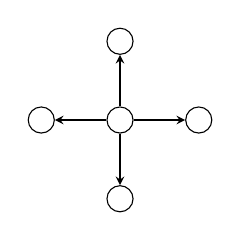
\begin{tikzpicture}[main/.style = {draw, circle}]

        \node[main] (10) {$ $};
        \node[main] (11) [below of=10] {$ $};
        \node[main] (12) [below of=11] {$ $};
        \node[main] (13) [right of=11] {$ $};
        \node[main] (14) [left of=11] {$ $};

        %\draw  node[fill,circle,scale=0.3]{} (0,0);

        \draw[-stealth] (11) -- (10);
        \draw[-stealth] (11) -- (12);
        \draw[-stealth] (11) -- (13);
        \draw[-stealth] (11) -- (14);

\end{tikzpicture}\end{center}
Chaque sommet, de coordonnées $(i,j)$, a pour voisins les sommets $(i,j-1),(i,j+1),(i-1,j),(i+1,j)$, et le poids des arêtes allant d'un sommet vers ses voisins est toujours égal à $1$. Le degré de chaque sommet est donc égal à $4$. Pour implémenter l'évolution au cours du temps d'un tel graphe, il est nécessaire de se limiter à un nombre fini de sommets. On considèrera donc uniquement les points de $\llbracket1,N\rrbracket^2$ pour un certain $N$. Dans ce cas, si un sommet instable $(i,j)$ est au bord du graphe, on fera comme s'il communiquait ses grains à quatre voisins, et que les grains de sable arrivant sur des sommets $(i,j) \notin \llbracket 1,N\rrbracket^2$ tombait ensuite dans un puits. Cela signifie en particulier que les sommets du bord peuvent s'effondrer sur l'extérieur (que nous appelerons puits dans la suite du rapport), mais que celui-ci ne peut s’écrouler sur les sommets du graphe.

Voici un exemple d'évolution d'un graphe de dimensions $3\times3$ pour le modèle du graphe feuille :
%La règle dynamique est la suivante, lorsqu’un site est à hauteur supérieure ou égale à 4, il s’effondre sur ses 4 voisins immédiats en distribuant à chacun un grain. Lorsqu'un site $x\in S$ où $S$ est l'ensemble des sommets du graphe appartient au bord du graphe $\partial \mathcal{G}$, les grains qu'il transmet à l'extérieur du graphe sont transmis à un puit, noté $s$ et sortent définitivement du système. Voici un exemple de stabilisation sur une grille $3\times 3$ pour ce graphe,
\begin{table}[htb]
    \hfill
    \begin{tabular}{c|c|c}
        0 & 0 & 0\tabularnewline
        \hline
        0 & 4 & 1\tabularnewline
        \hline
        0 & 4 & 1
    \end{tabular}
    \hfill
    \begin{tabular}{c|c|c}
        0 & 1 & 0\tabularnewline
        \hline
        1 & 1 & 2\tabularnewline
        \hline
        1 & 1 & 2
    \end{tabular}
    \hfill\null
    \caption{Configuration initialement instable, notée $\omega$ puis la stabilisée après un effondrement, notée $\mathfrak{s}(\omega)$.}
    \label{uca}
\end{table}

Voici un second exemple, modélisant un effondrement du haut vers le bas : on considère le graphe dont les sommets sont obtenus en tronquant $\mathbb{Z}^2$ selon le principe évoqué précédemment, et dont les arêtes sont conçues selon le schéma suivant, en mettant un poids égal à un sur chaque arête.
\begin{center} 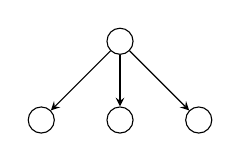
\begin{tikzpicture}[main/.style = {draw, circle}] 
    
        \node[main] (1) {$ $}; 
        \node[main] (2) [below of=1] {$ $};
        \node[main] (3) [left of=2] {$ $}; 
        \node[main] (4) [right of=2] {$ $};
        
        %\draw  node[fill,circle,scale=0.3]{} (0,0);
    
        \draw[-stealth] (1) -- (2);
        \draw[-stealth] (1) -- (3);
        \draw[-stealth] (1) -- (4);  
    \end{tikzpicture} 
\end{center}

Un sommet $(i,j)$ a alors pour voisins les sommets $(i-1,j-1), (i-1,j+1), (i-1,j)$, et le degré de chaque sommet est $3$.
Voici un exemple d'évolution d'un tel graphe, avec une configuration initiale comportant des sommets instables, et une configuration ne comportant que des sommets stables au bout de deux itérations :

    
\begin{table}[htb]
    \hfill
    \begin{tabular}{c|c|c}
        0 & 3 & 0\tabularnewline
        \hline
        1 & 2 & 1\tabularnewline
        \hline
        0 & 0 & 1
    \end{tabular}
    \hfill
    \begin{tabular}{c|c|c}
        0 & 0 & 0\tabularnewline
        \hline
        2 & 3 & 2\tabularnewline
        \hline
        0 & 0 & 1
    \end{tabular}
    \hfill
    \begin{tabular}{c|c|c}
        0 & 0 & 0\tabularnewline
        \hline
        2 & 0 & 2\tabularnewline
        \hline
        1 & 1 & 2
    \end{tabular}
    \hfill\null
    \caption{Configuration initialement instable puis la stabilisée après deux effondrements.}
    \label{uca}
\end{table}

Les modèles de piles abéliennes sont des systèmes dits à criticalité auto-organisée, c'est-à-dire évoluant  spontanément vers un état critique (en l'occurrence un état stable). Ils possèdent des propriétés intéressantes, tellles qu'une structure fractale, ainsi que des lois en puissance sur des grandeurs agrégées.

\section{Quelques exemples}
Dans ce qui suit, on appelle configuration la matrice contenant les hauteurs affectées aux différents sommets d'un graphe.
On admet provisoirement qu'étant donné un graphe $\mathcal{G}$, et la fonction unStab qui à une configuration $\omega$ sur ce graphe associe la configuration obtenue après une itération de la règle dynamique associée à ce graphe, dont le schéma général a été décrit précédemment, il existe, pour toute configuration affectant une hauteur à un nombre fini de sommets (ce qui est nécessairement le cas si on considère un graphe obtenu en tronquant $\mathbb{Z}^2$ pour ne conserver qu'un nombre fini de sommets, comme décrit avec l'exemple du graphe feuille), un nombre fini d'itérations au bout duquel le graphe se trouve dans une configuration où tous les sommets sont stables. On dit alors de la configuration qu'elle est stable. On note alors $\mathfrak{s}(\omega)$ la configuration stable obtenue après un nombre suffisant d'itérations de unStab, en partant de la configuration $\omega$. 

On appelle identité, et on note $I$, la configuration telle que, pour toute configuration $\omega$ sur le graphe $\mathcal{G}$, on ait : $\mathfrak{s}(I+\omega)=\mathfrak{s}(\omega)$. On a alors le résultat suivant : notant $c$ la configuration obtenue en affectant à chaque sommet d'un graphe $\mathcal{G}$ une hauteur égale à son degré (i.e. la plus petite hauteur rendant ce sommet instable, $\Delta_{x,x}$), on a $I=\mathfrak{s}(2c-\mathfrak{s}(2c))$. On utilise ce résultat pour coder un algorithme de calcul de l'identité pour le graphe suivant :
\begin{align*}
	\mathcal{G} = \{(X,X+\delta) : X\in\llbracket 1, N\rrbracket^2, \delta\in\{-1,1\}\times\{0\}\cup\{0\}\times\{-1,1\}\}
\end{align*}


Ce graphe est supposé connecté en ses bords à un extérieur appelé puits, comme expliqué dans la première partie de ce rapport.
On utilise le code suivant pour le calcul de l'identité.
\begin{lstlisting}
Hashtable <Integer, ArrayList<Integer>> gP = Graphes.grapheFeuille(N);
		int[] configuration = calculIdentiteDict(gP, false, true);
		rendu.save(PREFIXE + "--" + String.format("%03d", 0), configuration, N, N);
\end{lstlisting}
En affectant une couleur à chaque hauteur, on peut représenter graphiquement la configuration ainsi obtenue :

\begin{figure}[h]
	\centering
	\includegraphics[scale=0.5]{./out/identitefeuille.png}
\end{figure}

On peut également calculer l'identité pour un graphe plus élaboré : ainsi, soit le graphe obtenu en ôtant au graphe précédent l'intérieur d'une hyperbole (et en considérant que ce qu'on a ôté fait maintenant partie de ce qu'on appelle le puits) :
\begin{align*}
	\mathcal{G} = \{(X,X+\delta) : X=(x_1,x_2)\in\llbracket1,N\rrbracket^2 : x_1x_2\leq C, \delta\in \{-1,1\}\times \{0\}\cup\{0\}\times\{-1,1\}\} 
\end{align*}

Ce graphe est obtenu en utilisant l'instruction \textup{Graphes.grapheHyperbolique(C, Graphes.grapheFeuille(N))}. La fonction \textup{Graphes.grapheHyperbolique} est définie en utilisant la fonction \textup{grapheConditionnel} qui permet de réaliser l'intersection entre la structure d'un graphe et une condition sur les sommets de ce graphe (ici $x_1x_2\leq C$).
\begin{lstlisting}
     Hashtable <Integer, ArrayList<Integer>> gP = Graphes.grapheHyperbolique(10,Graphes.grapheFeuille(N));
        int[] configuration = calculIdentiteDict(gP, false, false);
        rendu.save(PREFIXE + "--" + String.format("%03d", 0), configuration, N,N);
\end{lstlisting}
\begin{figure}[h]
	\centering
	\includegraphics[scale=0.5]{./out/identitehyperbolique.png}
\end{figure}
Considérons à présent un troisième exemple : le graphe suivant est celui obtenu à partir du graphe feuille, en se limitant aux sommets appartenant à $\mathcal{B}_{\mathbb{Z}^2}(0,||.||_r,R)$, la boule de rayon $R$ de $\mathbb{Z}^2$, avec $||(i,j)||_r= (|i|^r+|j|^r)^{1/r}$ :
\begin{align*}
	\mathcal{G}(r) = \{(x,x+\delta) : x\in\mathcal{B}_{\mathbb{Z}^2}(0,||.||_r, R), \delta\in\{-1,1\}\times\{0\}\cup\{0\}\times\{-1,1\}\}
\end{align*}
Ce graphe est donné par \textup{Graphes.grapheCercle(R, Graphes.grapheFeuille(2*R), r)}, où \textup{Graphes.grapheCercle} est définie en utilisant la fonction \textup{grapheConditionnel}. Le code suivant renvoie les identités sur ce graphe pour $r \in\{0.5, 1, 1.5, 2, 2.5, 3\}$. 
\begin{lstlisting}
for (int k=0; k<6; k++) {
	Hashtable <Integer, ArrayList<Integer>> gP = Graphes.grapheCercle(N/2-1, Graphes.grapheFeuille(N), (k+1)*0.5);
	int[] configuration = calculIdentiteDict(gP, false, false);
	rendu.save(PREFIXE + "--" + String.format("%03d", k), configuration, N, N);
}
\end{lstlisting}
\begin{figure}[h]
\centering
\subfloat{{\includegraphics[scale=0.45]{/home/grothendieck/1A/ENSAE1A/info/out/avalancheXS--000.png}}}
\qquad
\subfloat{{\includegraphics[scale=0.45]{/home/grothendieck/1A/ENSAE1A/info/out/avalancheXS--001.png}}}
\qquad
\subfloat{{\includegraphics[scale=0.45]{/home/grothendieck/1A/ENSAE1A/info/out/avalancheXS--002.png}}}
\qquad
\subfloat{{\includegraphics[scale=0.45]{/home/grothendieck/1A/ENSAE1A/info/out/avalancheXS--003.png}}}
\qquad
\newline
\subfloat{{\includegraphics[scale=0.45]{/home/grothendieck/1A/ENSAE1A/info/out/avalancheXS--004.png}}}
\qquad
\subfloat{{\includegraphics[scale=0.45]{/home/grothendieck/1A/ENSAE1A/info/out/avalancheXS--005.png}}}
\end{figure}
\newpage
\section{Description de l'algorithme de stabilisation, preuve de terminaison et complexité}
Nous détaillons l'algorithme de stabilisation d'un graphe à partir d'une configuration de départ $\omega$ donnée.
\subsection{Pseudo-code}
\begin{algorithm}[H]
	initialisation : graphe $\mathcal{G}$, \\
	matrice laplacienne $\Delta$,\\ configuration $\omega$\\
	$\Sigma \leftarrow$ sitesInstables($\mathcal{G}$, $\Delta$, $ \omega$)\\
	\Tq{$\Sigma \neq \varnothing$} {
		unStab($\mathcal{G}$, $\Delta$, $\omega$, $\mathcal{S}$)\\
		$\Sigma \leftarrow$ sitesInstables($\mathcal{G}$, $ \Delta$, $\omega$) 
	}
\end{algorithm}

où la fonction unStab fait s'effondrer tous les sommets instables $x\in \Sigma$,\newline 
\begin{algorithm}[H]
	\Pour{$x\in\Sigma$} {
		$\omega(x) \leftarrow \omega(x)-\Delta_{x,x}$\\
		\Pour{$y\in \textup{Voisins}(x)$}{
			$\omega(y) \leftarrow \omega(y) - \Delta_{x,y}$
		}
	}
\end{algorithm}
On définit la laplacienne $\Delta$ du graphe de la façon suivante : pour $x$ et $y$ sommets du graphe $\mathcal{G}$, $\Delta_{x,y}= -p$ où $p$ est le poids de l'arête allant de $x$ vers $y$.  S'il n'y a pas d'arête de $x$ vers $y$, on pose $p=0$. Enfin, on pose $\Delta_{x,x}$ égal au degré de $x$.

\subsection{Preuve de terminaison}
La terminaison est assurée par l'existence, pour tout site $x\in S$ du graphe, d'un chemin partant de $x$ arrivant au puits $\mathcal{C}=(x\mapsto v_1\mapsto \ldots\mapsto s)$ à flux $-\sum_{v\in \mathcal{C}} \Delta_{x,v}$ strictement positif. 
\subsection{Complexité}
La principale difficulté réside dans l'évaluation du nombre d'étapes nécessaires à ce que $\Sigma$ se vide. Nous proposons ici une heuristique "à la physicienne" permettant d'évaluer ce temps car nous n'avons pas trouvé de ressource claire sur le net évaluant la complexité temporelle du modèle des piles abéliennes. 

%Notons $\partial \mathcal{G}$ le bord du graphe $G$, c'est-à-dire l'ensemble des sommets $x$ de $\mathcal{G}$ tels que $x\mapsto s$ où $s$ est l'évier. Pour $x\in\partial\mathcal{G}$, on note $-\Delta_{x,s}=d(x)>0$ la quantité de grains communiqués au puit $s$. On considère un partitionnement, $\partial \mathcal{G}_1,\ldots,\partial\mathcal{G}_k$,  de $\partial \mathcal{G}$ par la relation d'équivalence $x\sim y$ si et seulement si $d(x) = d(y) = d_i$.  Notons $\mu = (|\partial\mathcal{G}_1|,\ldots,|\partial\mathcal{G}_k|)$ et $D = (d_1,\ldots,d_k)^T$ alors pour des temps suffisamment longs (où le système est entrain de revenir à un équilibre en atteignant les bords), la quantité de sites instables $M_t = |\Sigma_t|$ vérifie $M_{t+1}\approx M_t(1-\mu.D/|\partial{\mathcal{G}}|)$. D'où en passant à des temps continus, $M_t \propto e^{-t\mu.D/|\partial{\mathcal{G}}|}$, l'heuristique nous dit donc que seuls les temps courts vont compter dans l'évaluation de la complexité temporelle. 

Notons $d = \max_{x\in S}\Delta_{x,x}$, le maximum des degrés sortants des sites. Il est aisé de voir que le temps mis par un grain pour atteindre le bord est proportionnel à une longueur caractéristique du graphe, par exemple, la taille d'un côté du graphe, disons $\sqrt{|S|}$. Ainsi, les temps courts sont proportionnels à $\sqrt{|S|}$. Pour qu'un grain sorte du système, il faut un temps $\sqrt{|S|}$. Le nombre de grains instables au cours du processus est majoré par une grandeur proportionnelle à $|S|$. On en déduit que $\Sigma$ se vide en un temps $O(|S|^{3/2})$. Le coefficient de proportionnalité peut être considéré comme quasiment constant en la géométrie du graphe (car localement, les graphes varient peu avec des degrés petits, $d$ est souvent de l'ordre de $3$ ou $4$). En pratique, on observe que lors du calcul de l'identité, $\Sigma$ se vide en un temps linéaire en $|S|$ avec un facteur de proportionnalité $c<1$.

Une lecture directe permet de voir que unStab est en $O(|\Sigma|\times d)$. On sait toutefois que $|\Sigma|\leq |S|$, donc unStab est en $O(|S|\times d)$. Comme nous n'avons pas réussi à évaluer l'évolution de la constante en fonction de $d$, on considérera $d$ comme constant pour obtenir une complexité en $O(|S|)$. La fonction siteInstables est en $O(|S|)$, ainsi la complexité temporelle de la fonction de stabilisation est en $O(|S|^{5/2})$. En reprenant les notations du code, où $n$ est la longueur d'un côté du graphe, on obtient $O(n^5)$. En pratique, pour le calcul de l'identité sur le graphe feuille, on est approximativement en $O(n^{4.1})$.

La complexité spatiale s'obtient en calculant la taille de la Hashtable représentant $\Delta$, elle est en $O(|S| d) = O(n^2 d)$.
\subsection{Concernant l'usage des Hashtables}
Nous avions tout d'abord envisagé de stocker la matrice laplacienne dans un tableau en deux dimensions. Cela occasionnait un coût en mémoire trop important. Or, les graphes que l'on considère contiennent peu d'arêtes par rapport au nombre de sommets (sinon l'on perdrait la localité des règles d'effondrement). Ainsi au lieu de stocker $|S|^2 = n^4$ valeurs dans une matrice, avec en grande majorité des $0$, nous avons préféré utiliser une table de hachage, qui nous permet de stocker directement la quantité $\Delta_{x,y}$ lorsqu'une arête de poids $-\Delta_{x,y}$ va de $x$ vers $y$, et de ne rien stocker lorsque $x$ n'est pas lié à $y$. On obtient alors la complexité spatiale calculée précédemment, $O(n^2d)$.
\subsection{Concernant des fonctions optimisées sur certains graphes}
Au cours de l'élaboration de notre programme, nous avons dû faire des compromis entre la concision du code et la vitesse d'exécution de celui-ci. La fonction permettant de lister les sites instables et qui fonctionne sur tous les graphes est celle qui s’exécute en $O(|S|)$. Elle calcule l'ensemble des sites $x$ instables. Sans hypothèse supplémentaire sur la localisation des sites instables à chaque étape, il n'est pas possible de faire mieux. 

Dans certains cas particuliers, il est cependant possible d’obtenir des solutions plus rapides. Ainsi, pour le graphe servant à modéliser un effondrement vers le bas présenté dans la première partie de ce document, il est clair, en numérotant les lignes de haut en bas ($t=1$ à $N$), que la présence d'un seul site instable en $t = 0$ implique que les sites instables à l'étape suivante se trouvent uniquement sur la ligne $t = 1$, puisque l'effondrement d’un sommet n'affecte que des sommets situés sur la ligne se trouvant immédiatement en-dessous de celui-ci. De la sorte, au lieu de vérifier la hauteur de chaque case du graphe, il suffit, à la $t$-ième itération, de vérifier la hauteur des sites sur la ligne correspondante $t-1$. La fonction unStab ainsi adaptée à ce graphe est de complexité linéaire en la largeur des lignes, ainsi elle nous permet de gagner au moins un facteur $\mathcal{O}(\sqrt{|S|}) = O(n)$. 
De plus, en utilisant un théorème que l'on verra par la suite, on sait que la probabilité qu'un effondrement atteigne une ligne $t$ ou plus est proportionnelle à $1/\sqrt{t}$. Ainsi, une proportion $p$ des configurations générées aléatoirement et dérangées en $t=0$ se stabilisent en un temps $t$ inférieur à $T\approx C/(1-p)^2$ avec $C< 1$ (avec $C = p_0^2$ et $p_0$ la probabilité qu'une configuration dure un temps $t\geq 2$, $p_0$ est facilement calculable). 
Comme à chaque étape $t$,  $|\Sigma|\leq dt =3t$, on sait que UnStab est en $O(t)=O((1-p)^{-2})$, qui est un coût constant en la taille du graphe. Cela permet d'obtenir une complexité en  $O(\sqrt{|S|})=O(n)$, avec une constante de proportionnalité qui évolue en fonction de $p$, en $(1-p)^{-4}$. C'est un coût sous-linéaire en la taille du graphe !
Pour cette raison, vous trouverez dans le code des fonctions avec différents suffixes, tels que DN pour "Downward neighbours". Celles-ci sont adaptées aux graphes qui admettent une direction d'effondrement vers le bas.
\section{Loi en puissance du flux carré moyen}
Reprenons le graphe introduit au début qui modélise un effondrement dirigé vers le bas, on pose
\begin{align*}
\mathcal{G}(E, \varphi) = \{(s,s+(\delta,1))_{\textup{de poids } \varphi_\delta} : \delta\in E, s=(x,t)\in\mathbb{Z}\times\mathbb{N}\}
\end{align*}

L'exemple donné au départ correspond à $E= \{-1,0,1\}$ et $\varphi = (1, 1, 1)$. L'objectif est d'étudier l'évolution d'une configuration tirée uniformément après un effondrement. Le principal théorème que nous avons démontré est que dans certaines bonnes conditions, ici vérifiées, le flux carré moyen, c'est-à-dire le carré du nombre de site instables à l'étape $t$ de l'effondrement, défini par $\Phi(t) = \mathbb{E}\bigg(\sum_{x\in\mathbb{Z}} \mathds{1}((x,t) \textup{s'effondre })\bigg)^2$ est, pour une certaine constante $\gamma$ calculable, tel que
	\begin{align*}
		\Phi(t) \sim \frac{1}{\gamma}\sqrt{\frac{t}{\pi}}
	\end{align*}

L'expression prévue pour le graphe d'introduction est $\Phi(t) \sim \sqrt{\frac{32 t}{3\pi}}$. Le code suivant permet de calculer une approximation du flux carré moyen.  
\begin{lstlisting}
        float[] f = fluxcarremoyen3neighbours(N, largeur, temps);
\end{lstlisting}

Après tracé des points ainsi obtenus, on constate la validité du théorème, 
\begin{figure}[h]
	\centering
	\includegraphics[scale=0.8]{/home/grothendieck/tipe/wwp.png}
\end{figure}

La probabilité qu'une avalanche s'étend plus loin que sur $t$ ligne est proportionnelle à $1/\sqrt{t}$ (voir le compte-rendu mathématique pour les références). On vérifie ce théorème en calculant un histogramme de la distribution de la taille des effondrements puis en calculant la fonction de survie empirique.
\begin{lstlisting}
Hashtable<Integer, Integer> resultat = histogramme3(10000, M,N);
\end{lstlisting}

On obtient la fonction de survie empirique et la courbe théorique d'expression $p_0/\sqrt{t}$ suivants
\begin{figure}[h]
	\centering
	\includegraphics[scale=0.8]{/home/grothendieck/tipe/wwpp.png}
\end{figure}
\section{Conclusion}
Nous avons présenté le modèle général des piles abéliennes sur un graphe quelconque. Nous l'avons implémenté (calcul de stabilisation, de l'identité, rendu visuel) ainsi que différentes méthodes pour générer des graphes particuliers. Enfin, à l'aide d'une heuristique ainsi que de résultats probabilistes, nous avons mené un calcul de complexité de nos algorithmes.

\end{document}
